\chapter{Linux kernel continuous integration}
\section{Context}
\subsection{Linux}
Linux is an operating system kernel (or simply kernel) created by Linus Torvalds and its source code was released in 1991 under a Free and Open Source license. After requests to remove the limitation on commercialization established by the current license, he ultimately released the source code under the GPL license\footnote{\url{https://www.kernel.org/pub/linux/kernel/Historic/old-versions/RELNOTES-0.12}} in 1992.

The Linux kernel is the biggest Open Source software with its 21 millions lines of code, 4000 contributors and several thousands of supported architectures. Such a big project needs people which are guarantors of the quality of the code and the respect of different rules (such as the coding style for example). These people are called maintainers and are specialized in a certain part of the Linux kernel, called a subsystem.

With a project this big and that segmented, it is hard to guarantee the modifications applied to the code source do not break the kernel especially when, in its 4.6 version, it averaged 11600 lines added, 5800 removed, and 2000 modified per day\footnote{\url{https://www.linux.com/news/greg-kroah-hartman-gives-inside-look-largest-fastest-software-project-all}}.

The Open Source Software biggest strength is in its openness. Everyone can audit the code to find security flaws or bugs and fix them or notify the community of these bugs. Most importantly, companies do not need to reinvent the wheel, they can reuse freely the most tried and tested software programs in the world.

\subsubsection{Contributions}

When one wants to upstream a code change in the Linux kernel source code, one has to follow a set of rules defined for the Linux kernel. This set of rules\footnote{\url{https://www.kernel.org/doc/Documentation/SubmittingPatches}} asks to:
\begin{itemize}
  \item extensively describe the code changes,
  \item separate all changes in small different \textit{patches},
  \item check indentation, coding style, comments of patches,
  \item take time to chose the persons to which the patches will be sent,
  \item respond to review comments,
  \item sign patches;
\end{itemize}

Once one has formatted its patches accordingly to the different rules, one has to send its patches for reviews to maintainers of all subsystems impacted by the changes, as well as their mailing lists.

\begin{figure}[H]
  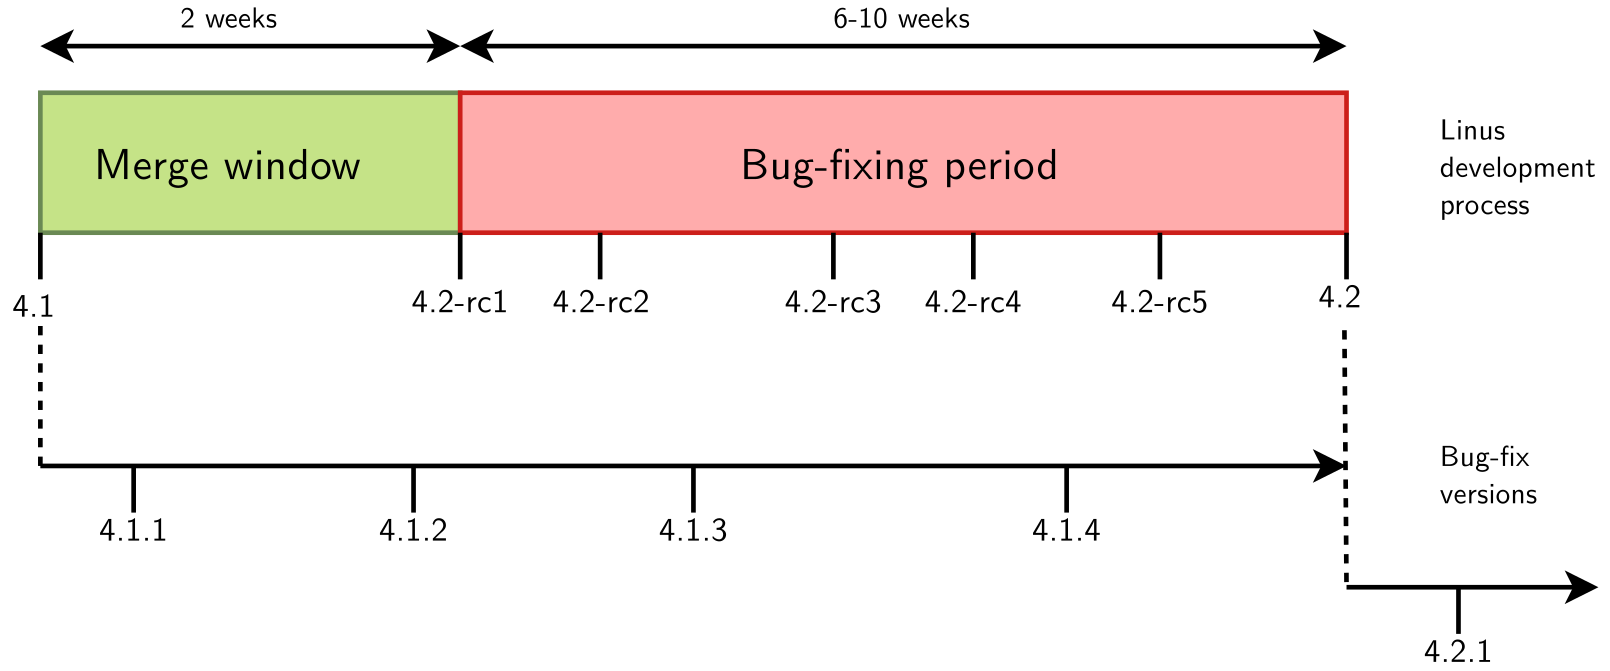
\includegraphics[width=\textwidth]{kernel-merge.png}
  \caption{Development schedule of the Linux kernel}
\end{figure}

The Linux kernel has a rather simple development schedule:
\begin{itemize}
  \item 2 weeks for the merge window,

During these two weeks, patches validated by the community prior to this period are merged to the upstreaming version of the Linux kernel.

  \item 6 to 10 weeks for the bug-fixing window,

During these few weeks, only important bug fixes and bug fixes for new features added during the merge window should be submitted to the community for the next version. This is also the period when the patches for new functionalities for the version after the next version are submitted.
\end{itemize}

Patches will be discussed via the mailing lists and once they are validated by maintainers, the latter will then merge the patches into their own git repository in branches destined for the Linux kernel version currently in development or the next one. The goal of these branches specific to each subsystem is to ease the merging of patches in the Linux kernel mainline version. Another git repository called linux-next\footnote{\url{https://git.kernel.org/cgit/linux/kernel/git/next/linux-next.git/}}, or simply next, is used to make intermediate test releases by automatically merging all subsystems' branches to the latest version of the Linux kernel. It allows to find merge failures and bugs before merging to the Linux kernel mainline version. During the merge window, Linus Torlads will merge all subsystem maintainers' git branches creating the first Release Candidate, or rc1, version of the next Linux kernel version.

Some vendors work differently with the Linux kernel. They usually forks (make a copy) of the Linux kernel git repository and makes tremendous changes in the source code without sending the changes for reviews to the community. Often, they do not update regularly their version to match the Linux kernel latest version which results in a complete nightmare when the vendor finally decide to upstream their modifications. This induces also that a board might only work with the vendor Linux kernel which does not contain the Linux kernel new functionalities or bug fixes (such as security fixes).

\subsubsection{Files built when compiling the Linux kernel}

When compiling the Linux kernel, some files are created:
\begin{itemize}
  \item the kernel image, which can be of different format, for example:

\begin{itemize}
  \item Image, which is the format for 64-bits ARM platforms,
  \item zImage, which is the format for all other platforms,
  \item uImage, which is a format specific to U-Boot bootloader, adding a header to specify the entry and load addresses in RAM of the kernel image;
\end{itemize}

  \item Device Tree Blobs, only created for ARM (32 or 64 bits) and PowerPC platforms;
\end{itemize}

The Device Tree, as its name suggests, is a tree of devices and a representation of hardware devices and buses which are present in a board and are not discoverable at runtime. This file is compiled beside the Linux kernel with the Device Tree Compiler and a change in its code does neither affect the kernel nor requires a rebuild of the kernel. A Device Tree Blob is created once the Device Tree has been compiled and has to be used in conjunction with a compiled kernel or the kernel will not be able to boot. A Device Tree is specific to one board but can inherit components' definition from Device Trees includes.

The Device Tree is a file organized like a tree, with a root node, bus nodes and devices nodes. The root node typically contains a \textit{cpus} node describing each CPU in the system, a \textit{memory} node defining the location and size of the RAM, an \textit{aliases} node specifying shortcuts to some nodes, and nodes describing SoC buses such as USB, i\textsuperscript{2}c or SPI and on-board devices such as LEDs, eMMC, SD card reader, Ethernet port or power regulators.

Two kernels differ by their configuration file (which drivers to build inkernel or as modules for example), their targeted architecture and the Device Trees compiled with it.

\subsection{Free Electrons' use case}
Some of Free Electrons' clients ask help to upstream a driver to the Linux kernel source code. Since Linux is FOSS (Free and Open Source Software), everyone can modify the code of this driver to add functionality or to fix bugs but it can also introduce new bugs because developers only test their code on the boards they own, often not the ones we own. Free Electrons' engineers need to continuously keep an eye on part of codes used by or developed for a client. Several clients also ask to follow the whole life-cycle of the project (from its early development stages to its discontinuity) so engineers have to keep track of all modifications of the kernel that might break the product.

\section{State of the art}
Since the kernel supports several thousands of different platforms, when a developer writes new code for the kernel, he cannot test his code on all the platforms and usually tests only on the platforms he owns. Before merging its code to the kernel source code, some users or other developers might test it on other platforms or in other configurations but it is rather rare. Furthermore, the only way to guarantee a modification works on all impacted platforms is to build the kernel in all its configurations and test on all these platforms if the kernel boots. This is extremely tedious and time consuming.

As explained above, there is currently no way to automatically discover a regression in the kernel beside Intel's 0-day\footnote{\url{https://01.org/lkp}} for x86 platforms. The only way to detect a regression for other platforms is when a user of the kernel performs an audit or is using the kernel in a certain configuration so that he discovers a bug. The software developed by Intel called 0-day which is a building test robot provides little help by taking patches from different mailing lists, applying them one by one to different branches and testing the Linux kernel can be properly built with the modifications included in the patch.

It is the role of a maintainer to guarantee the stability and the working of the subsystem he's in charge. However, since he hasn't all the platforms impacted by his subsystem, the only thing he can do is to look for common errors in the code and try to find corner cases.

The main goal of KernelCI project is to implement a continuous integration in the kernel so build or boot failures are detected before reaching the end users. There already are several labs contributing to the project: several from Linaro and few from KernelCI founders. However, they are often expensive (i.e. the Linaro's lab uses several 500\$ APC PDU\footnote{Power Distribution Unit} systems to control the power of boards) and we do not want to put that much money in a lab so one of the challenges is to have working, cheap (but not hackish) solutions.

At Free Electrons, we also love to contribute to free software programs and we are very proud to be part of the effort to bring continuous integration to the kernel.

\section{Project}
\subsection{Continuous integration in Linux kernel}

Continuous integration is the process of automated building and testing of a software when one or multiple changes have been made to its source code, and then reporting of the results. The main benefit of continuous integration is to detect as soon as possible regressions in the code so they could be identified and corrected quickly, ideally before being in a production environment.

Because of Linux's well-known ability to run on numerous different platforms and the obvious impossibility for developers to test changes on all these platforms, continuous integration has a big role to play in Linux kernel development and maintenance.

Continuous integration is made up of three different steps:
\begin{itemize}
  \item building the software which in our case is the Linux kernel,
  \item testing the software,
  \item reporting the tests results;
\end{itemize}

\begin{figure}[H]
  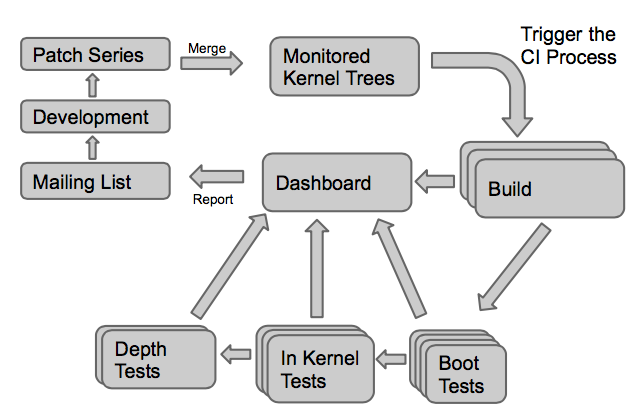
\includegraphics[width=\textwidth]{kernel-ci-overview.png}
  \caption{KernelCI complete process}
\end{figure}

\subsection{Building the kernel}

Something has to trigger the build of the Linux kernel. It could be either changes in a git branch or in a whole git repository or patches sent to mailing lists. Most of these tracking means are not automatic and have to be scheduled to check for changes once in a while. We can tweak the granularity of the tracking by controlling the period of time between two scheduled checks.

KernelCI is permanently tracking around a dozen of kernel git repositories. Each hour, KernelCI checks if the git repositories have been updated and if so, KernelCI builds from the last commit the kernel for ARM, ARM64 and x86 platforms in many configurations and their associated Device Trees. Then it stores all these builds in a publicly available storage\footnote{\url{https://storage.kernelci.org/}}.

\subsection{Testing the kernel}

KernelCI is not in charge of this part of continuous integration but is rather delegating this step to the software installed in organization's or individual's labs.

\subsubsection{Software choices}

At this moment, two software programs are known to work with KernelCI: Linaro Automated Validation Architecture (LAVA)\footnote{\url{http://www.linaro.org/initiatives/lava/}} and pyboot\footnote{\url{https://github.com/khilman/pyboot}}. pyboot is going deprecated so LAVA is highly preferred for new labs. LAVA was created early 2012 to meet Linaro's developers' needs to continuously test their work before delivering it to their client. Note that KernelCI does not solely interact with pyboot or LAVA since it offers an API\footnote{\url{https://api.kernelci.org/}}, so if none meets your needs, go ahead and make your own!

\subsubsection{What is LAVA?}

LAVA is a self-hosted software, organized in a server-dispatcher model, for controlling boards to automate boot, bootloader and user-space testing. The server receives \textit{jobs} specifying what to test, how and on which boards to run those tests, and transmits those jobs to the dispatcher linked to the specified board. The dispatcher applies all modifications on the kernel image needed to make it boot on the said board and then fully interacts with it through the serial. There is only one LAVA server but there could be one or more dispatchers, each one having its own boards. Since we plan to have around 50 boards in our lab, we have only one computer which is used as both LAVA server and dispatcher.

Since LAVA has to fully and autonomously control boards, it needs to:
\begin{itemize}
  \item interact with the board through serial connection,
  \item control the power supply to reset the board (in case of a crashed kernel or when a job has finished to limit useless power consumption),
  \item know the commands needed to boot the kernel from the bootloader,
  \item serve files (kernel, Device Tree Blob (DTB), rootfs) to the board.
\end{itemize}

The first three means are given to LAVA by per-board configuration files. The latter is done by the LAVA dispatcher in charge of the board which downloads files specified in the job and copy them to a directory accessible by the board through TFTP.

LAVA organizes the lab in \textit{device types} and in \textit{devices}. All identical devices are from the same device type and share the same configuration file. A device type configuration file contains the set of instructions to run in the bootloader to boot the kernel (e.g.: how and where to load files) and the bootloader configuration (e.g.: can it boot zImages or only uImages). A device configuration file stores the commands run by a dispatcher to interact with the device: how to connect to serial, how to power it on and off. LAVA interacts with devices via external tools: it has support for conmux or telnet to communicate via serial and power commands can be executed by custom scripts or pdudaemon\footnote{\url{https://github.com/Linaro/pdudaemon}} for example.

\subsubsection{Control power supply}

Some labs use expensive ($\sim$500\$) systems to control the power supply of each board but we do not want to put that much money into a small part of our lab. Therefore, we went for Ethernet-controlled relays. We could have used USB-controlled relays as well but there are already a lot of USB connections going on with the serial connection for each board so we chose the former. It is possible to communicate with these Ethernet-controlled relays using TCP frames.

I first developed our own software to control boards' power supplies but I figured out it would be better to contribute to pdudaemon. pdudaemon is developed by Linaro and is widely tried and tested for almost 3 years now. It works in a server-client fashion: client sends the request (power on or off a board) to the server which queues it if there is more than one power-control pending operation and then executes the requested operation. To control boards' power, we use several Devantech ETH008 Ethernet-controlled relays for which I had to add support in pdudaemon\footnote{\url{https://github.com/Linaro/pdudaemon/pull/9}}, which was made straight-forward thanks to pdudaemon's drivers model implementation. The server is handled by a daemon while the client is called by LAVA dispatchers to send power-control requests to pdudaemon's server.

\subsubsection{Connect to serial}

As advised in LAVA's installation guide\footnote{\url{https://validation.linaro.org/static/docs/v1/installation.html\#setting-up-serial-connections-to-lava-devices}}, we went with telnet and ser2net\footnote{\url{http://linux.die.net/man/8/ser2net}} to connect to boards' serial. ser2net basically opens a Linux device and allows to interact with it through TCP sockets on a defined port. A LAVA dispatcher will then launch a telnet client to connect to boards' serial. Because of the well-known fact that Linux devices' name might change between reboots, I had to use udev rules in order to guarantee the serial we connect to is the one we want to connect to.

\subsubsection{Actual testing}

Now that LAVA knows how to handle devices, it has to run jobs on those devices. LAVA jobs contain which images to boot (kernel, DTB, rootfs), what kind of tests to run when in user space and where to find them. A job is strongly linked to a device type since it contains the kernel and DTB specifically built for this device type. LAVA has the ability to run jobs simultaneously, meaning jobs can be run on different device types at the same time. Since devices in the same device type are assumed to behave like each other, when a job requests a certain device type, it will only run on one device of this device type.

\begin{figure}[H]
  \center
  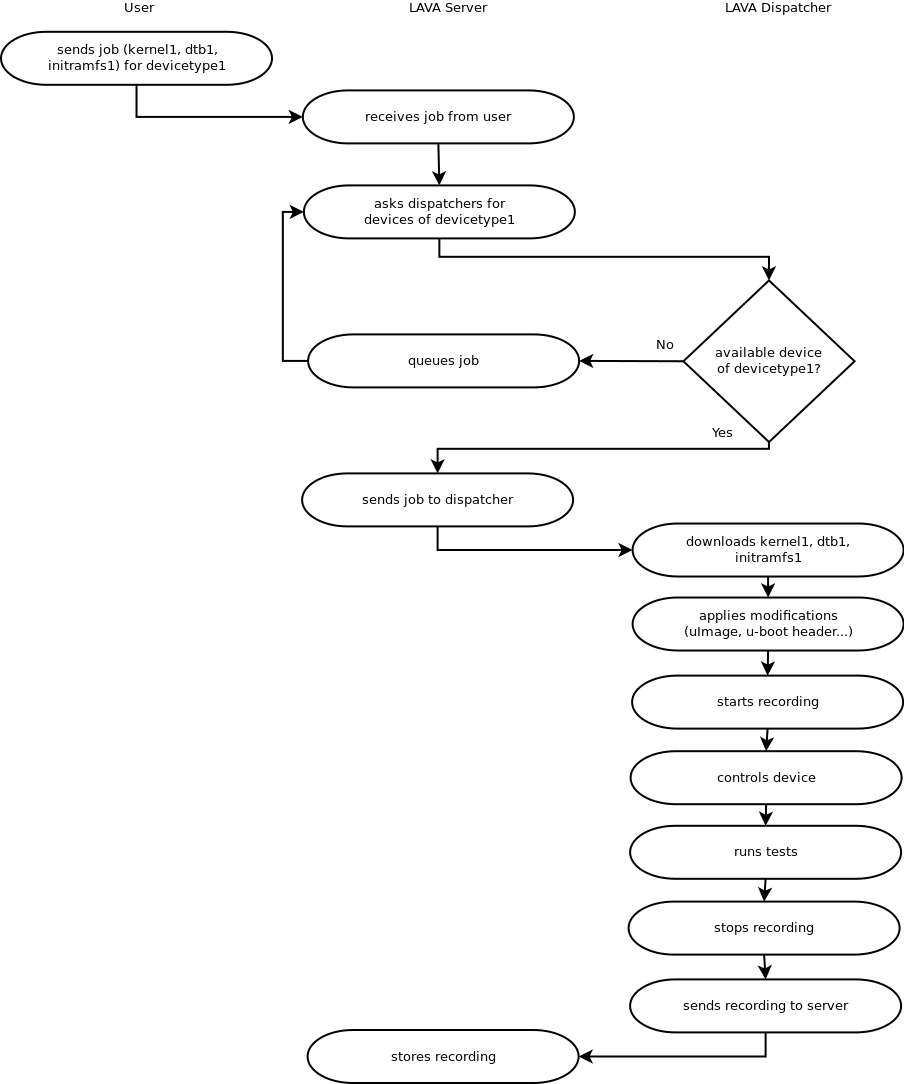
\includegraphics[width=0.815\textwidth]{user-server-dispatcher.png}
  \caption{LAVA server and dispatcher complete process}
\end{figure}

As you can see, everything is automated only after the user has sent the job. Yet, to achieve full automation, we have to automate the sending of jobs too which is made possible thanks to LAVA's API. Now, the only remaining barrier is to build kernels on git notifications or crontabs for example, create tests and send them to LAVA via its API.

KernelCI is taking care of sending jobs to contributing labs to run minimal testing on latest versions of the kernel. To send jobs to LAVA's API, it uses lava-ci\footnote{\url{https://github.com/kernelci/lava-ci/}} for which we added and will continue to add the support for all boards. When KernelCI has finished to build a kernel, it creates a job for all boards represented by a Device Tree in the different configurations of this kernel.

\subsection{Reporting test results}

After KernelCI has built the kernel, sent jobs to contributing labs and LAVA (or another software) has run the jobs, KernelCI will then get the tests results from the labs, aggregate them on its website and notify maintainers of errors via a mailing list.

\subsection{Hardware infrastructure}

\subsubsection{Specifications}

Our lab is supposed to take place in Free Electrons' offices in a 100cm wide space. The room in which the lab will take place is separated from the office by a 200cm high and 75cm wide door and we thought it would be a good idea to build the lab a little smaller so if we move out of this office a day, we do not have to completely disassemble it but rather slide it through the doors.

Finally, Free Electrons' engineers filled a spreadsheet with all boards they wanted to have in the lab and their particularities regarding which connectors are used for the serial communication and the power supply. We reached a total of 48 boards to put into the lab. Among those boards, we can distinguish two different types:
\begin{itemize}
  \item boards which are powered by an ATX power supply,
  \item boards which are powered by chargers;
\end{itemize}

In addition to needing a full ATX power supply, the first type of boards often has a huge motherboard. These boards sometimes also embed extension ports such as PCI-e, making their height bigger. The biggest height we could find was 25cm for a board with a PCI-e device plugged in.

We also wanted the lab to be easy to use and evolve. Sometimes, engineers will need to take a board out of the lab or to add one. The easier the process is, the better the lab is. Building the lab with drawers seemed to be the easiest, cheapest and quickest way to make our lab modular. Since we have two types of boards, one taking a lot of room in a drawer, we thought it would be a good idea to separate both types in different drawers. \textit{Big drawers} would host the boards which need a separate ATX power supply while the \textit{small drawers} would host the smallest boards.\\
Typically, considering the size limitations of the lab, our drawers would have a maximal size of 95x70cm. We determined we could put 8 small boards on a small drawer and up to 4 big boards on a big drawer. Since we went with drawers, we had to think of a system to limit the number of cables connecting the server and the hardware components on each drawer so it is easy to slide the drawer.\\
Given the maximal height of the lab to be a bit less than 200cm and the minimal height allowed for a drawer to be 25cm, we knew we could have 8 drawers in our lab. From the spreadsheet containing all the boards supposed to be in the lab, we eventually decided there would be 3 \textit{big drawers} for up to 12 \textit{big} boards and 5 \textit{small drawers} for up to 40 \textit{small} or \textit{medium-sized} boards.

\begin{figure}
  \centering
  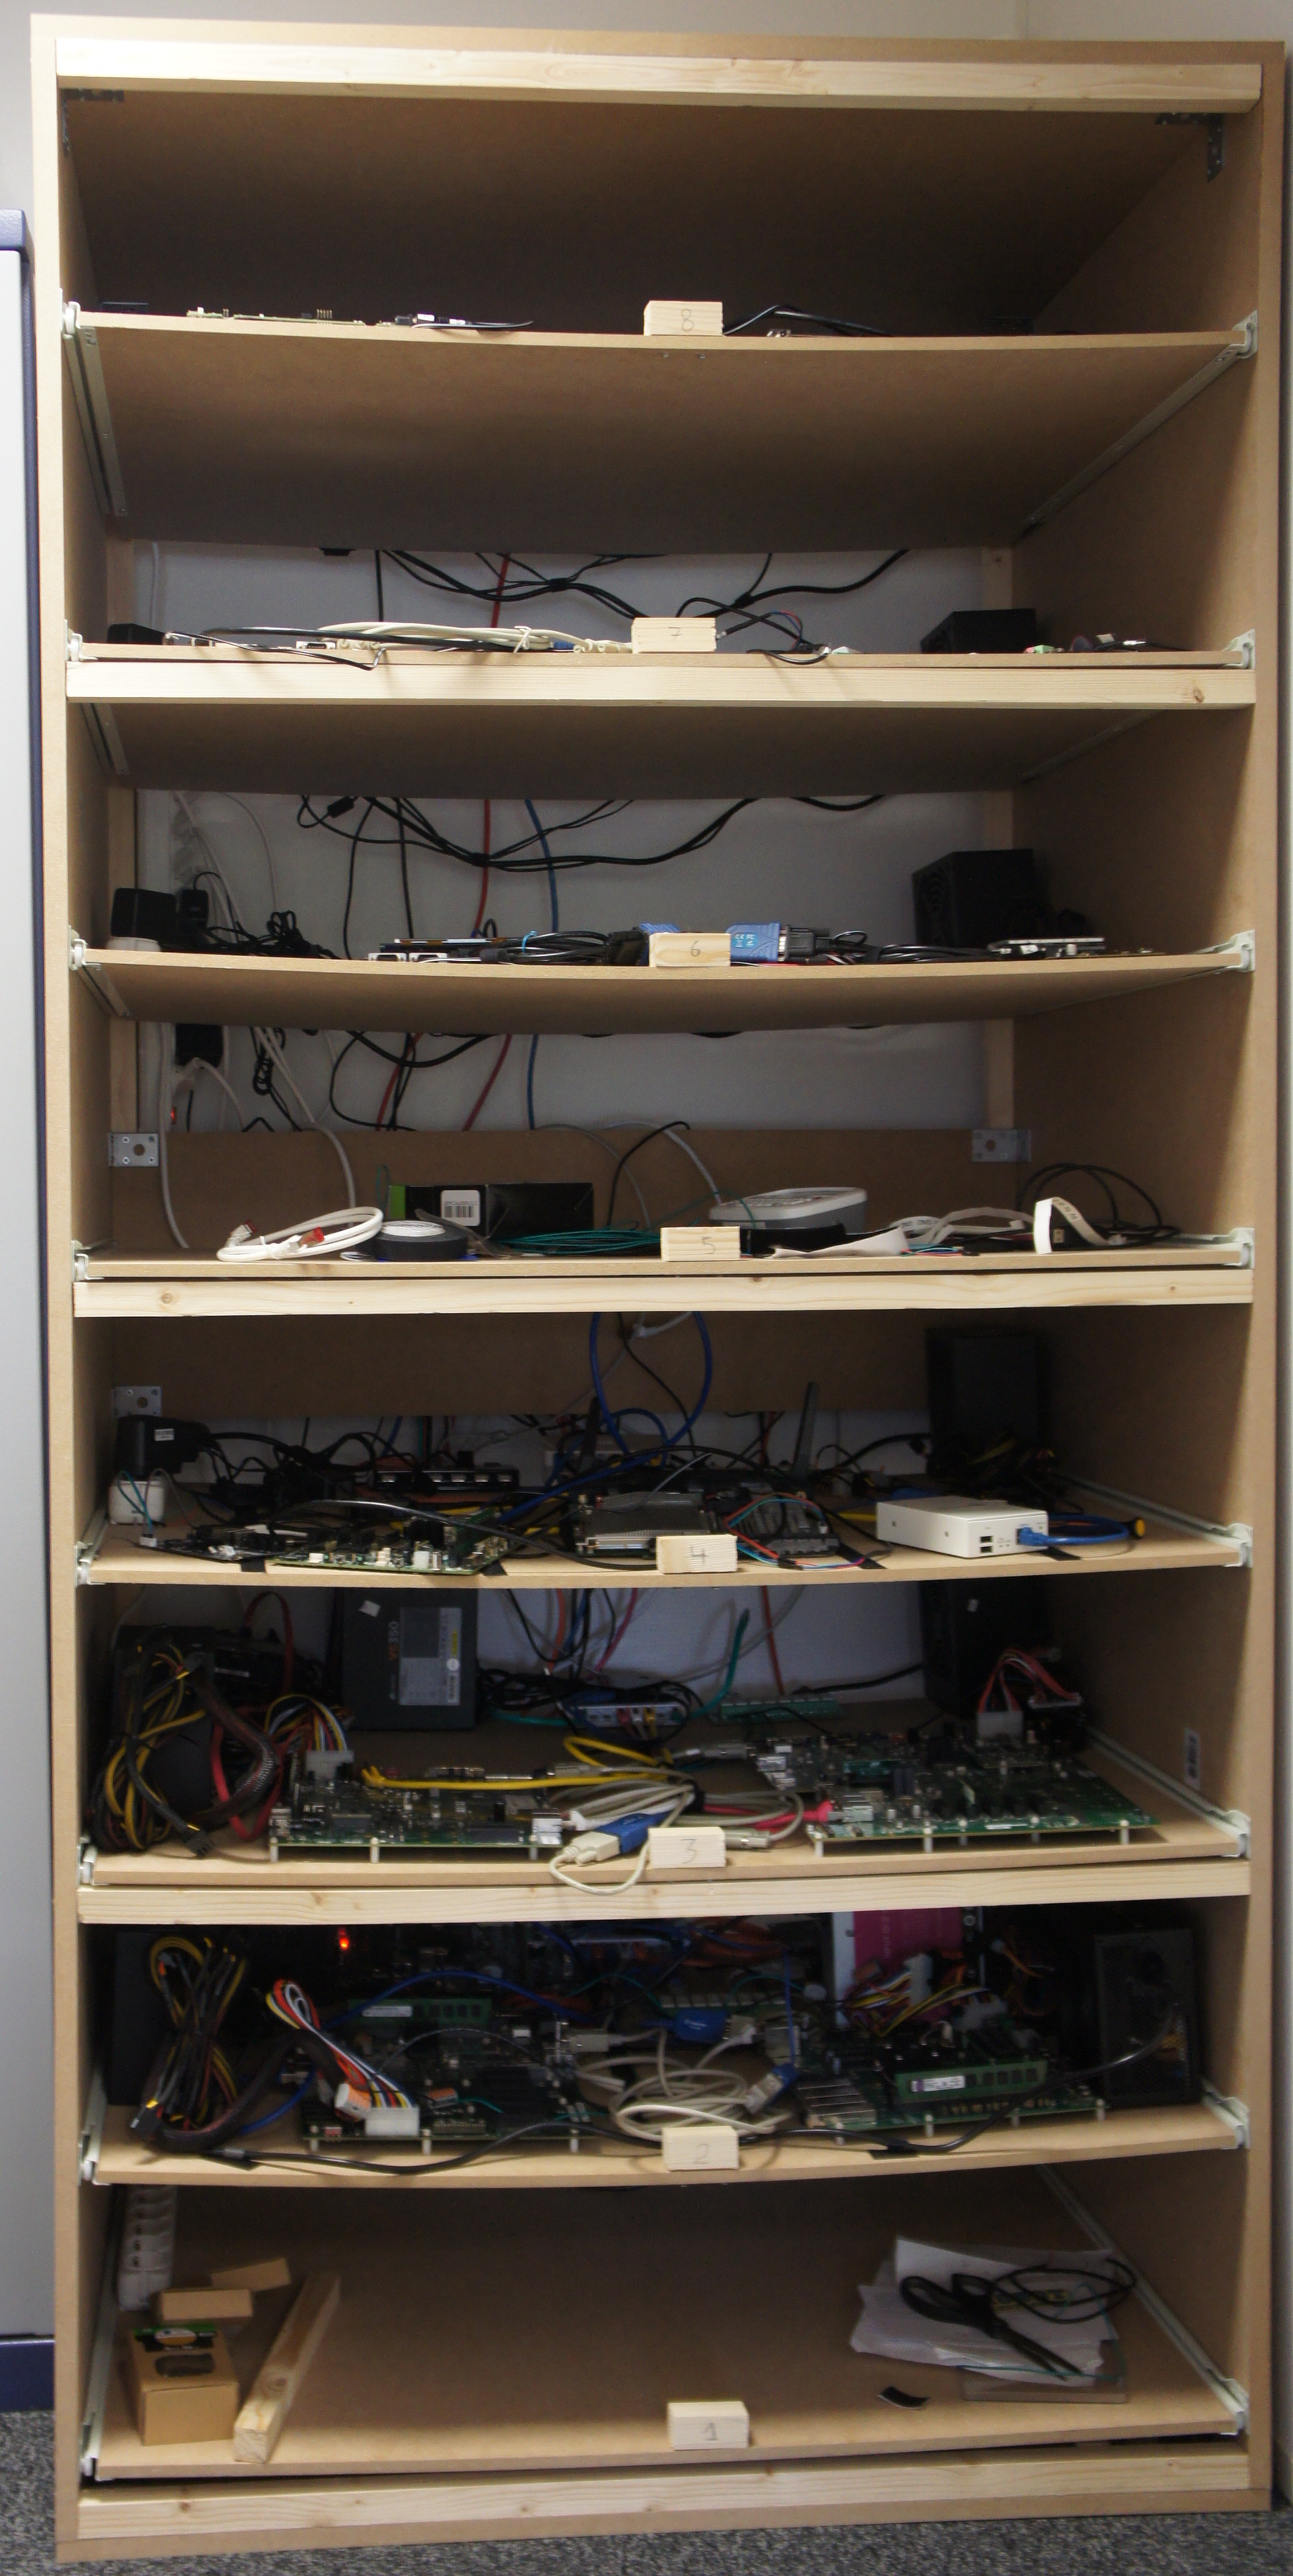
\includegraphics[width=0.7\textwidth]{lab.JPG}
  \caption{Free Electrons' 8 drawers lab}
\end{figure}

To organize our drawers and ease their evolution, we needed to cleanly guide the cables to each board while making it easy to remove them in any occasion. Some boards are also so tiny and light, the rigid cables connected to the board imposed the place where the board will stay. Also, we needed to keep the power supplies and other hardware materials in place. Therefore, we needed an easy-to-remove way to guide cables and also maintain boards and heavy materials at a given place. We thought scratch bands were an excellent choice:

\begin{itemize}
  \item easy to reposition,
  \item unharmful to cables and boards (neither electrostatic nor made of metal),
  \item strong enough to hold boards and heavy materials in place,
  \item cheap and easy to find;
\end{itemize}

Therefore, we needed a scratch band with one side to stick to the drawer and the other in either hooks or loops material, and a second scratch band with one side in hook material and the other in loop material. The second scratch band would circle cables and boards hooking to itself and to the first scratch thus keeping them in place. The first scratch would also be used to stick the power supplies, the switches, USB hubs and Ethernet-controlled relays to the drawer.

\begin{figure}[H]
  \centering
  \begin{minipage}[b]{0.45\textwidth}
    
\includegraphics[width=\textwidth]{scratch_hooks.jpg}
    \caption{Scratch hooks (CC-BY-3.0 Alexander Klink)}
  \end{minipage}
  \hfill
  \begin{minipage}[b]{0.45\textwidth}
    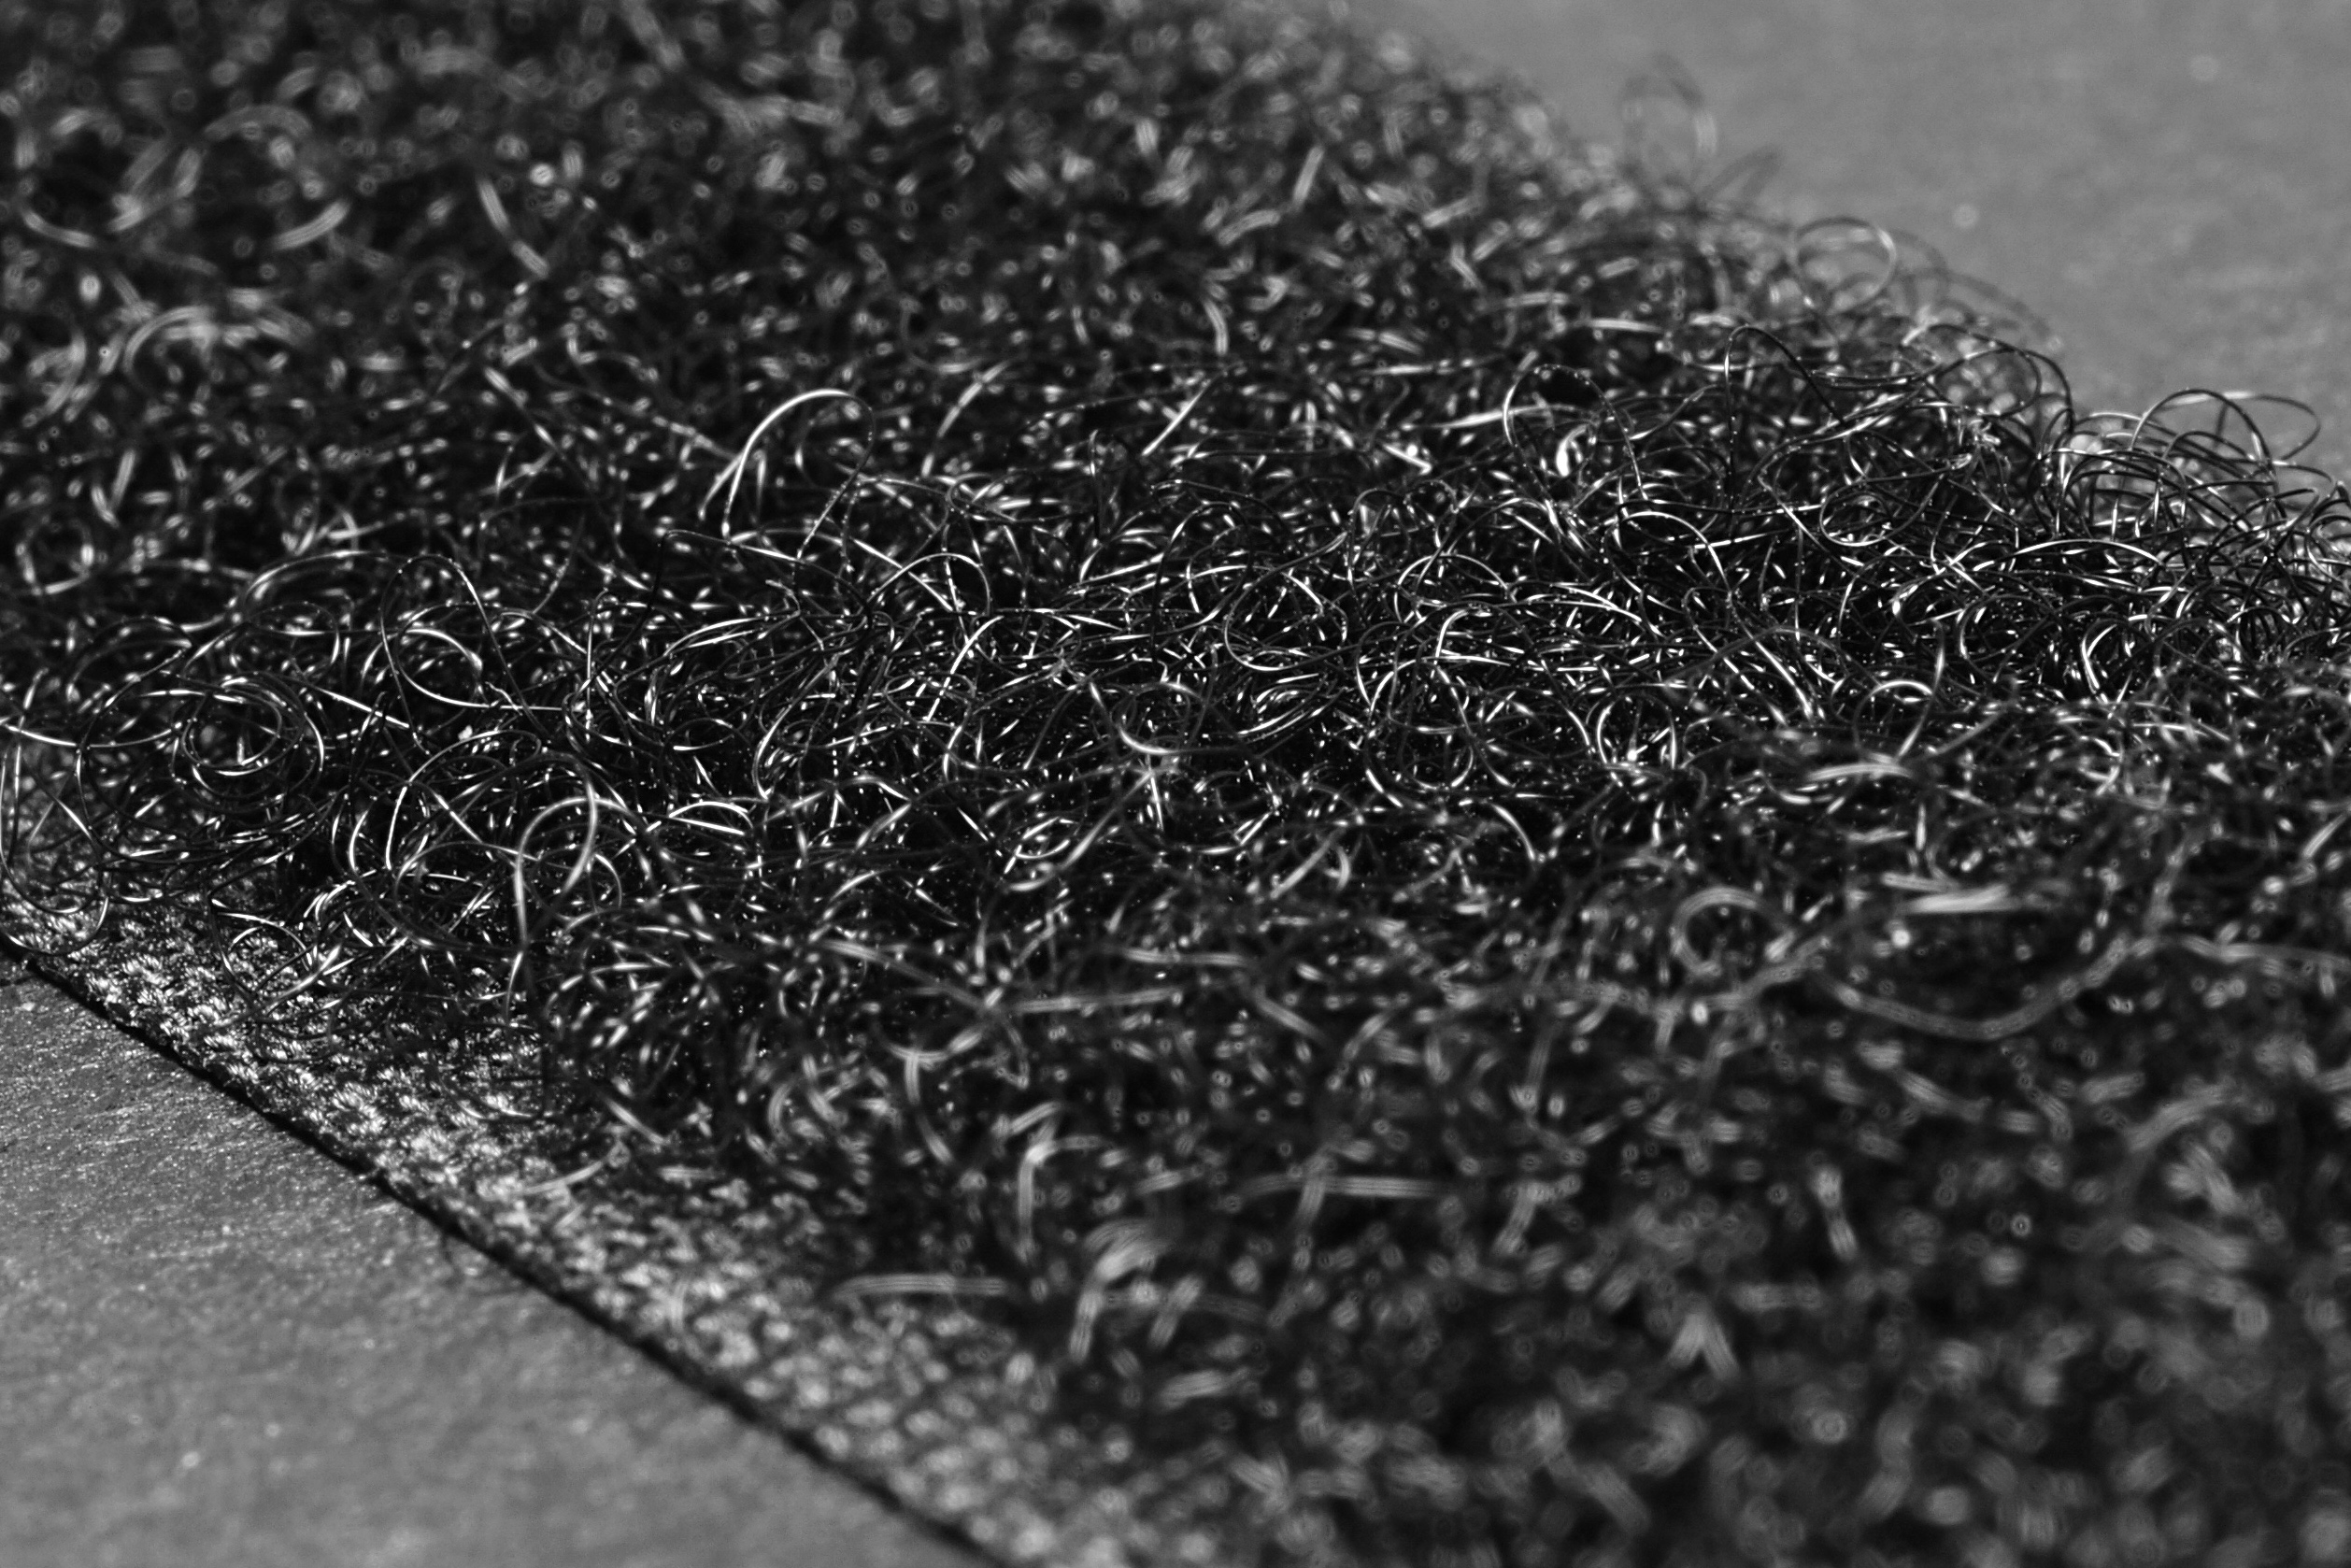
\includegraphics[width=\textwidth]{scratch_loops.jpg}
    \caption{Scratch loops (CC-BY-3.0 Alexander Klink)}
  \end{minipage}
\end{figure}

Furthermore, since the lab would host a server and a lot of boards and power supplies, potentially producing a lot of heat, we had to keep the lab as open as it can be while making sure it is strong enough to hold the drawers.

After that, we had to meet LAVA hardware requirements.

\subsubsection{Connect to serial}

Serial connections are mostly handled via USB on host side but there are many different connectors on target side (in our lab, we have 6 different connectors: DE9, microUSB, miniUSB, separate male pins, separate female pins and USB-B).

In a LAVA setup with several dispatchers, each dispatcher has to be physically connected to all of the boards it's in charge of. In our case, the server hosts the LAVA master and dispatcher all at once. Therefore, our server had to have a physical connection with each of the 50 boards present in the lab. The need for USB hubs was then obvious.

Since we wanted as less cables connecting the server and the drawers as possible, we decided to have one USB hub per drawer, be it a \textit{big drawer} or a \textit{small drawer}. In a \textit{small drawer}, up to 8 boards can be present, meaning the hub needs at least 8 USB ports. In a \textit{big drawer}, up to 4 serial connections can be needed so smaller and more common USB hubs can do the work. However, since the serial connection may draw some current on the USB port, we wanted all of our USB hub to be powered with a dedicated power supply.

All USB hubs are then connected to a main USB hub which in turn is connected to our server.

\subsubsection{Control power supply}

LAVA needs to control each board's power to be able to automatically power on or off a board. It will power on the board when it needs to test a new kernel on it and power it off at the end of the test or when the kernel has frozen or could not boot at all.

We thought of two different ways to control power supplies:
\begin{itemize}
  \item having a power supply for each board connected to an Ethernet-controlled multi-socket which can power on or off each socket individually,
  \item having one big power supply for all the boards, split the output wire between all boards and connect it to Ethernet-controlled relays which open or close the connection between the power supply and the board;
\end{itemize}

In \textit{small drawers}, up to 8 boards need a separate power supply. Professional controllable multi-sockets are too expensive, too big and too heavy (sometimes rackable) and often offer US sockets or \textit{kettle cords}\footnote{\url{https://en.wikipedia.org/wiki/IEC\_60320\#C13.2FC14\_coupler}} only which means we have to buy adapters to switch from European to US sockets or to connect the kettle cord to the board's charger. More affordable controllable multi-sockets are available on the market but they often include only 6 sockets which is not enough for our \textit{small drawers}. The first option seems out of our scope.

The second option would need a power supply with enough amperage to power all boards at the same time. In the future, we may want to attach hard drives to some boards for cryptography or RAID tests for example. Spin-up of hard drives draws a lot of current so we have to add some amps to the minimal needed amperage.\\
Amongst our boards some need 5 Volts inputs while other need 12 Volts inputs. This requirement would induce to have two different power supplies (one delivering 5V and the other 12V) or a power supply which can deliver both at the same time. When gathering information and experiences from different labs, Kevin Hilman, one of KernelCI's founders, told us he uses ATX power supplies to power both 5V and 12V boards. He splits both outputs and plugs them in an Ethernet-controlled relay to individually open or close the power circuit to each board. This was the best product we could think of to power the boards since desktop ATX power supplies often deliver a lot of current to power multiple graphic cards, hard drives and the processor. So we could use one ATX power supply per \textit{small drawer} to handle all the power for all boards in this drawer.

\begin{figure}[H]
  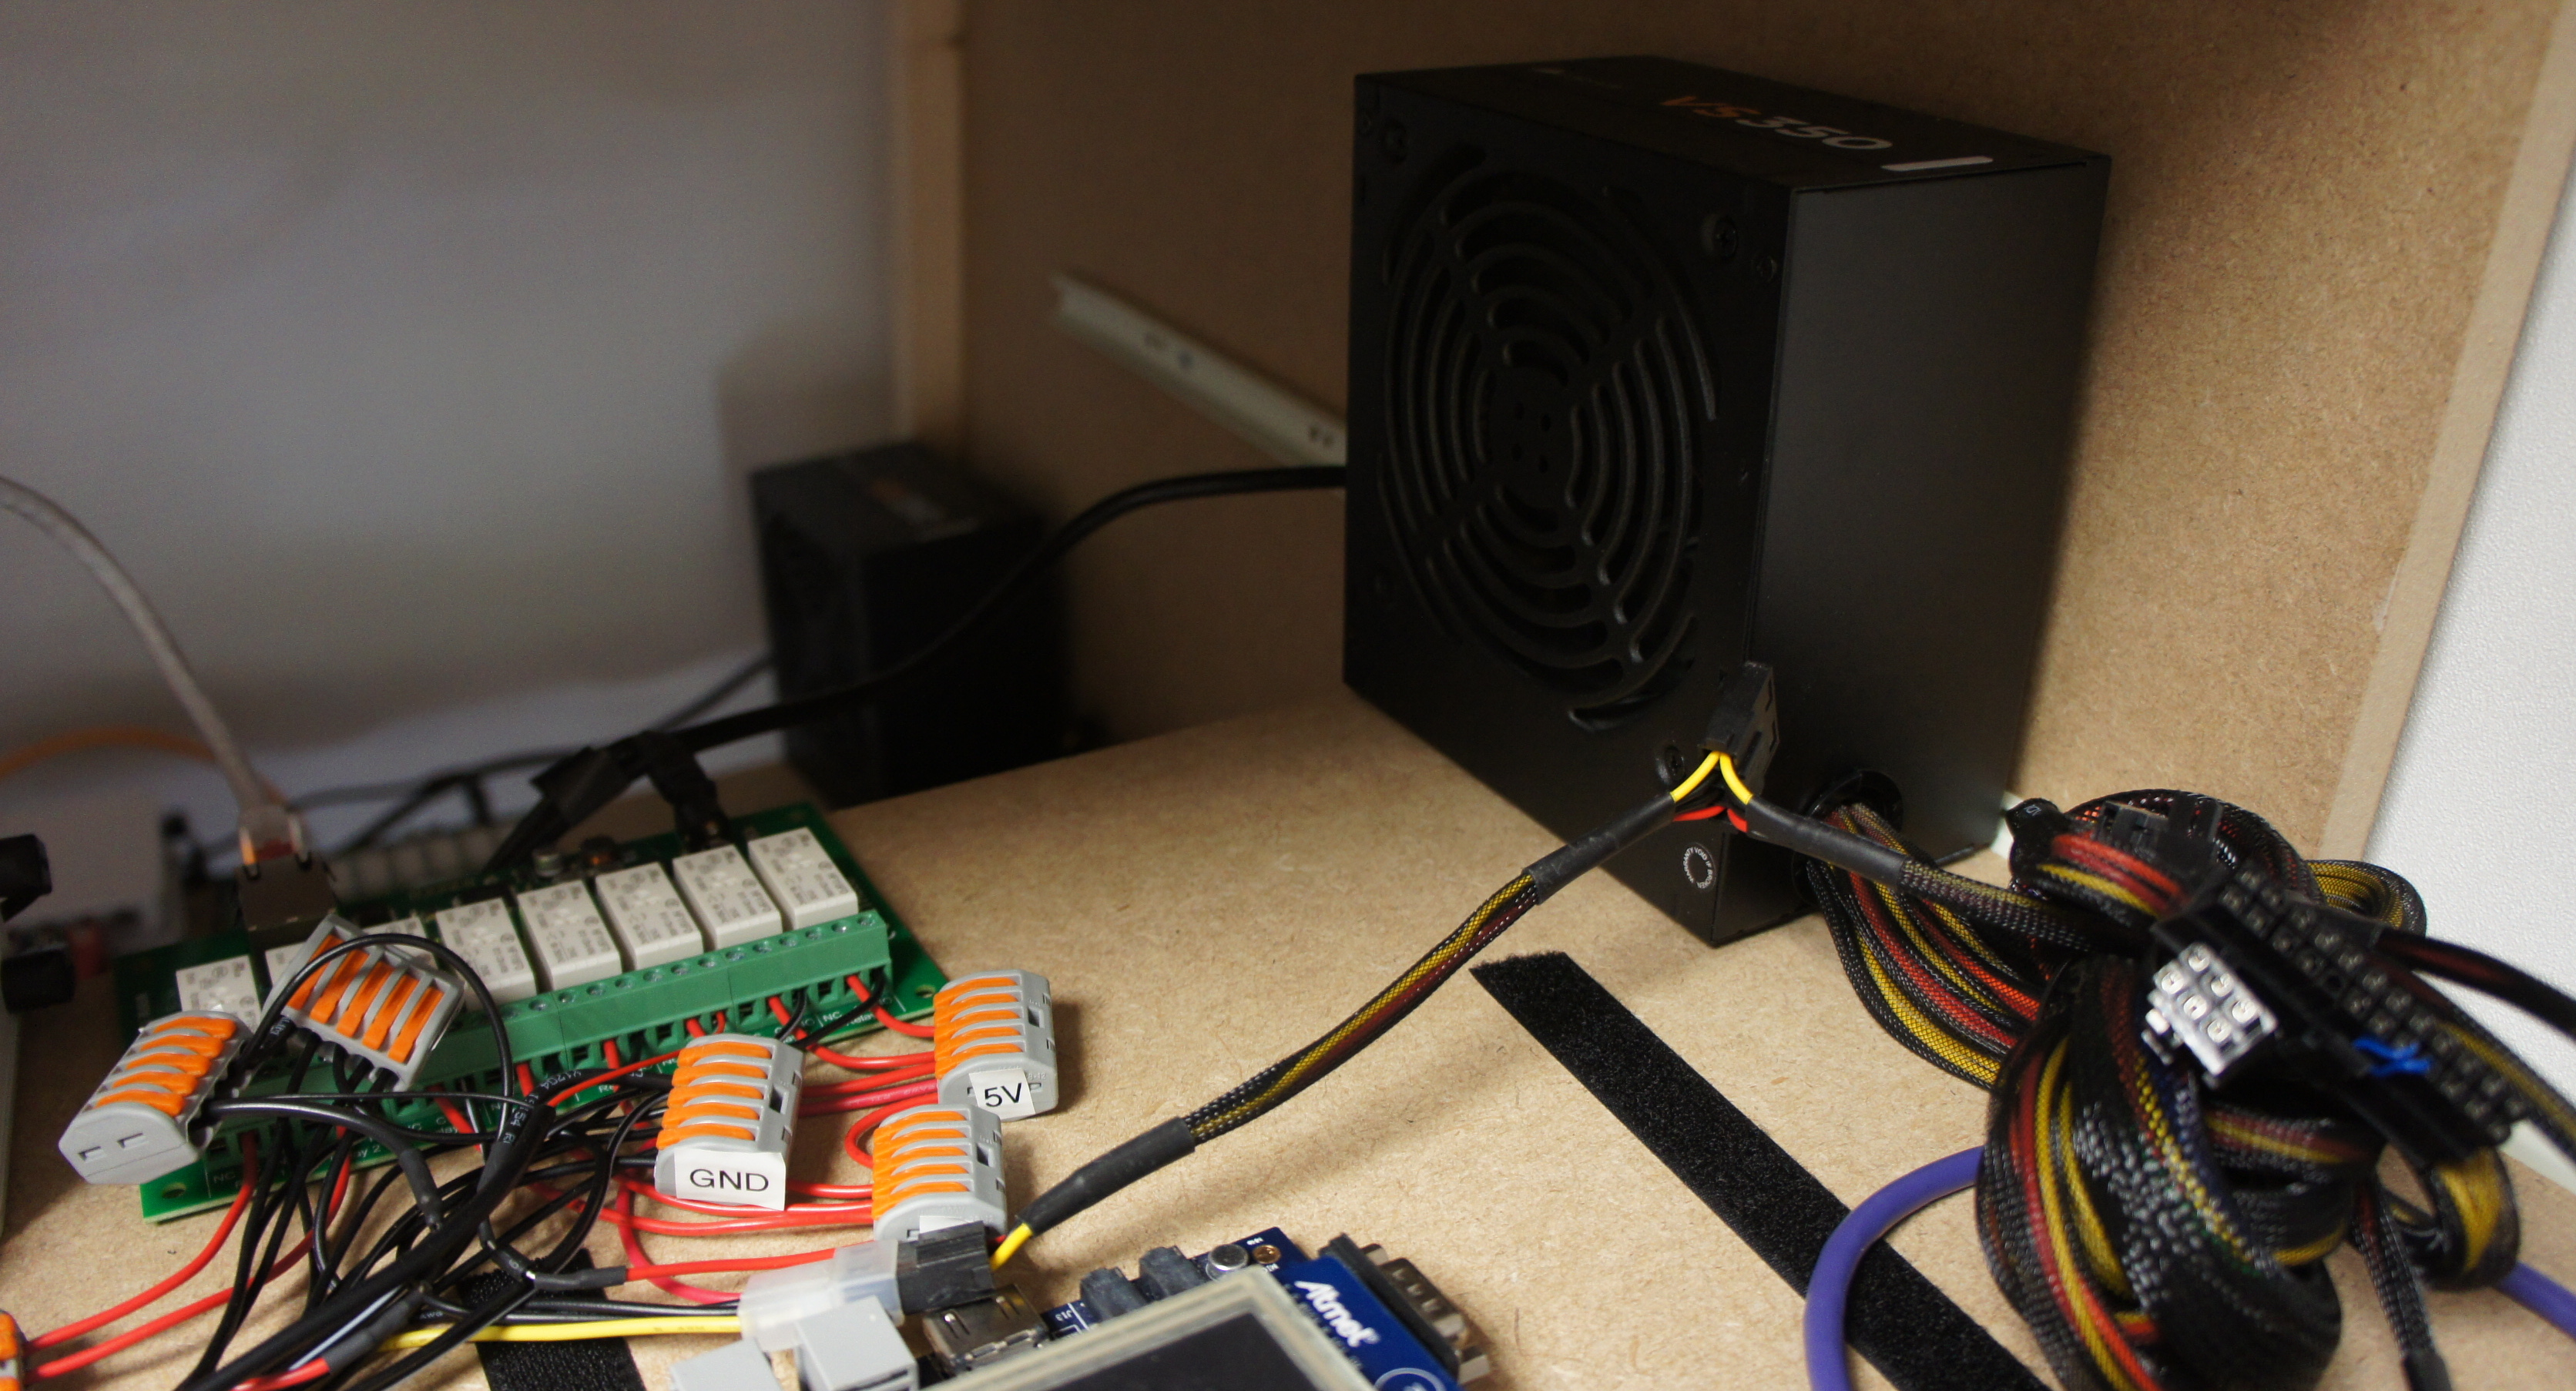
\includegraphics[width=\textwidth]{power_supply.JPG}
  \caption{Splitting ATX power supply 5V, 12V and ground outputs}
\end{figure}

However, there was still one problem: an ATX power supply is always powered but does not always deliver power. This is a way to spare electricity when the desktop is not used thus not needing the ATX power supply to deliver power. When we press the power button on a desktop, it sends a signal to the ATX power supply to start delivering power. The boards in our \textit{small drawers} are not supposed to be powered with an ATX power supply so they do not know how to send this signal to the power supply. Moreover, the signal has to be sent on a separate wire which is not connected to any of these boards. This signal is called \textit{PS\_ON\#}\footnote{\url{http://www.formfactors.org/developer/specs/atx2\_2.pdf}} and is supposed to be applied to the 16\textsuperscript{th} pin (normally green wire) of the 24-pins connector of the power supply. When this pin is connected to the ground, the power supply turns on.

Since the Ethernet-controlled relays make sure the power circuit to the boards is open when the boards are powered off, we can permanently turn on the power supply by putting the pin to the ground for \textit{small drawers}.

However, it is different for boards which need a separate ATX power supply, i.e. in \textit{big drawers}. In this case, the board is powered when the switch on the board is in the \textit{ON} position. This switch basically takes the ground from the power supply and connects it to the 16\textsuperscript{th} pin when it is in the \textit{ON} position. We cannot manually switch the board's switch each time we need to reset the power of the boards since LAVA needs to be autonomous. The solution was to split the ground, cut the green wire from the ATX power supply before the connector and plug both in the same Ethernet-controlled relay which will connect them together only when needed, thus powering the ATX power supply.

By definition, a power supply does not deliver a stable voltage but rather guarantees the delivered voltage will be within a certain range. However, the power supply might still malfunction and deliver a voltage too high for the board thus burning it. This is a big problem, besides fire hazard, because boards are expensive and sometimes owned only once. To try to prevent such problems, we added TVS\footnote{Transient-voltage-suppression diode} diodes for each voltage output in each drawer. These diodes will absorb all the voltage when it exceeds the maximum authorized value and explode and are connected in parallel in the circuit to protect\footnote{\url{https://en.wikipedia.org/wiki/Transient-voltage-suppression\_diode}}.

\subsubsection{Serve files}

LAVA has two ways of serving files to a board: via TFTP\footnote{\url{https://en.wikipedia.org/wiki/Trivial\_File\_Transfer\_Protocol}} or via fastboot\footnote{\url{https://wiki.cyanogenmod.org/w/Doc:\_fastboot\_intro}}. Since fastboot is using the USB protocol, it is by definition slower than TFTP which uses the UDP protocol. Thus, when possible, we use TFTP over fastboot for speed sake. Moreover, fastboot is often not supported due to an old version of the bootloader for example.

Since TFTP is using UDP protocol to serve files to each board, we needed to connect the boards and the server to the same network. Because we wanted the least possible cables between drawers and the server and also because an at-least 52-ports switch is unbelievably expensive, we decided to have one switch per drawer which will be connected to a main switch to which the server will be connected.

Each board needs its own Ethernet cable, meaning 8 ports are reserved on a \textit{small drawer}'s switch for boards' network connection while 4 ports are reserved on a \textit{big drawer}'s switch for its own boards. Each drawer also needs to reserve one port for the Ethernet-controlled relays and one port used to connect to the main switch. Therefore, switches present on \textit{small drawers} will need at least 10 ports while switches on \textit{big drawers} will need 6 ports.\\
We might want in the future to perform speed tests on network interfaces of boards and thus, we decided to go only with gigabit switches. With this in mind, there were two choices for switches on \textit{small drawers}: one 16-ports switch or two 8-ports switches. Since we already needed one 8-ports switch per \textit{big drawer} and the fact that two 8-ports switches were cheaper than one 16-ports switch, we chose to have only 8-ports switches for drawers.

We settled for a 16-ports gigabit switch as the main switch since it connects 8 switches, the server and the ISP\footnote{Internet Service Provider} box.

For network cables, we quickly calculated the maximal length of a link in a drawer is 1m while we need a minimum of 2m for cables connecting drawer's switches and the main switch and multiple very short cables for connecting switches in \textit{small drawers} and the Ethernet-controlled relays. Therefore we bought around 80 meters of network cables.

\begin{figure}[H]
  \centering
  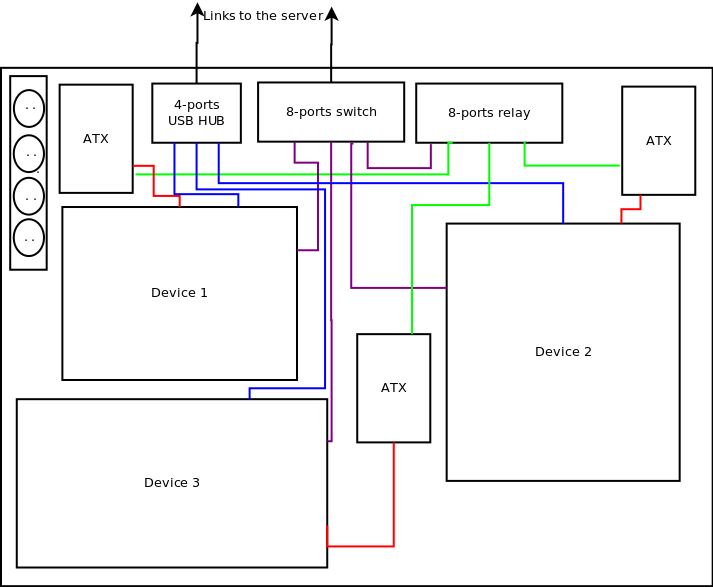
\includegraphics[width=0.7\textwidth]{big-drawer-scheme.png}
  \caption{\textit{Big drawer} example scheme}
\end{figure}
\begin{figure}[H]
  \includegraphics[width=\textwidth]{big_drawer.JPG}
  \caption{\textit{Big drawer} in the lab}
\end{figure}
\begin{figure}[H]
  \centering
  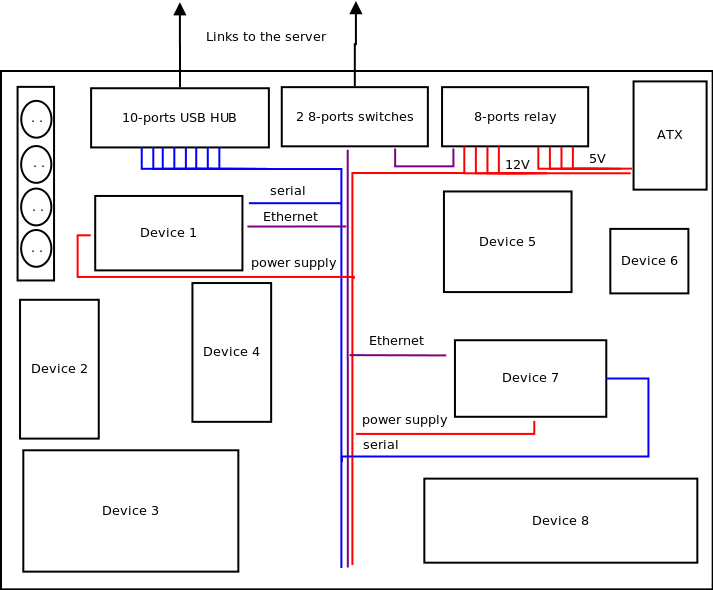
\includegraphics[width=0.7\textwidth]{small-drawer-scheme.png}
  \caption{\textit{Small drawer} example scheme}
\end{figure}
\begin{figure}[H]
  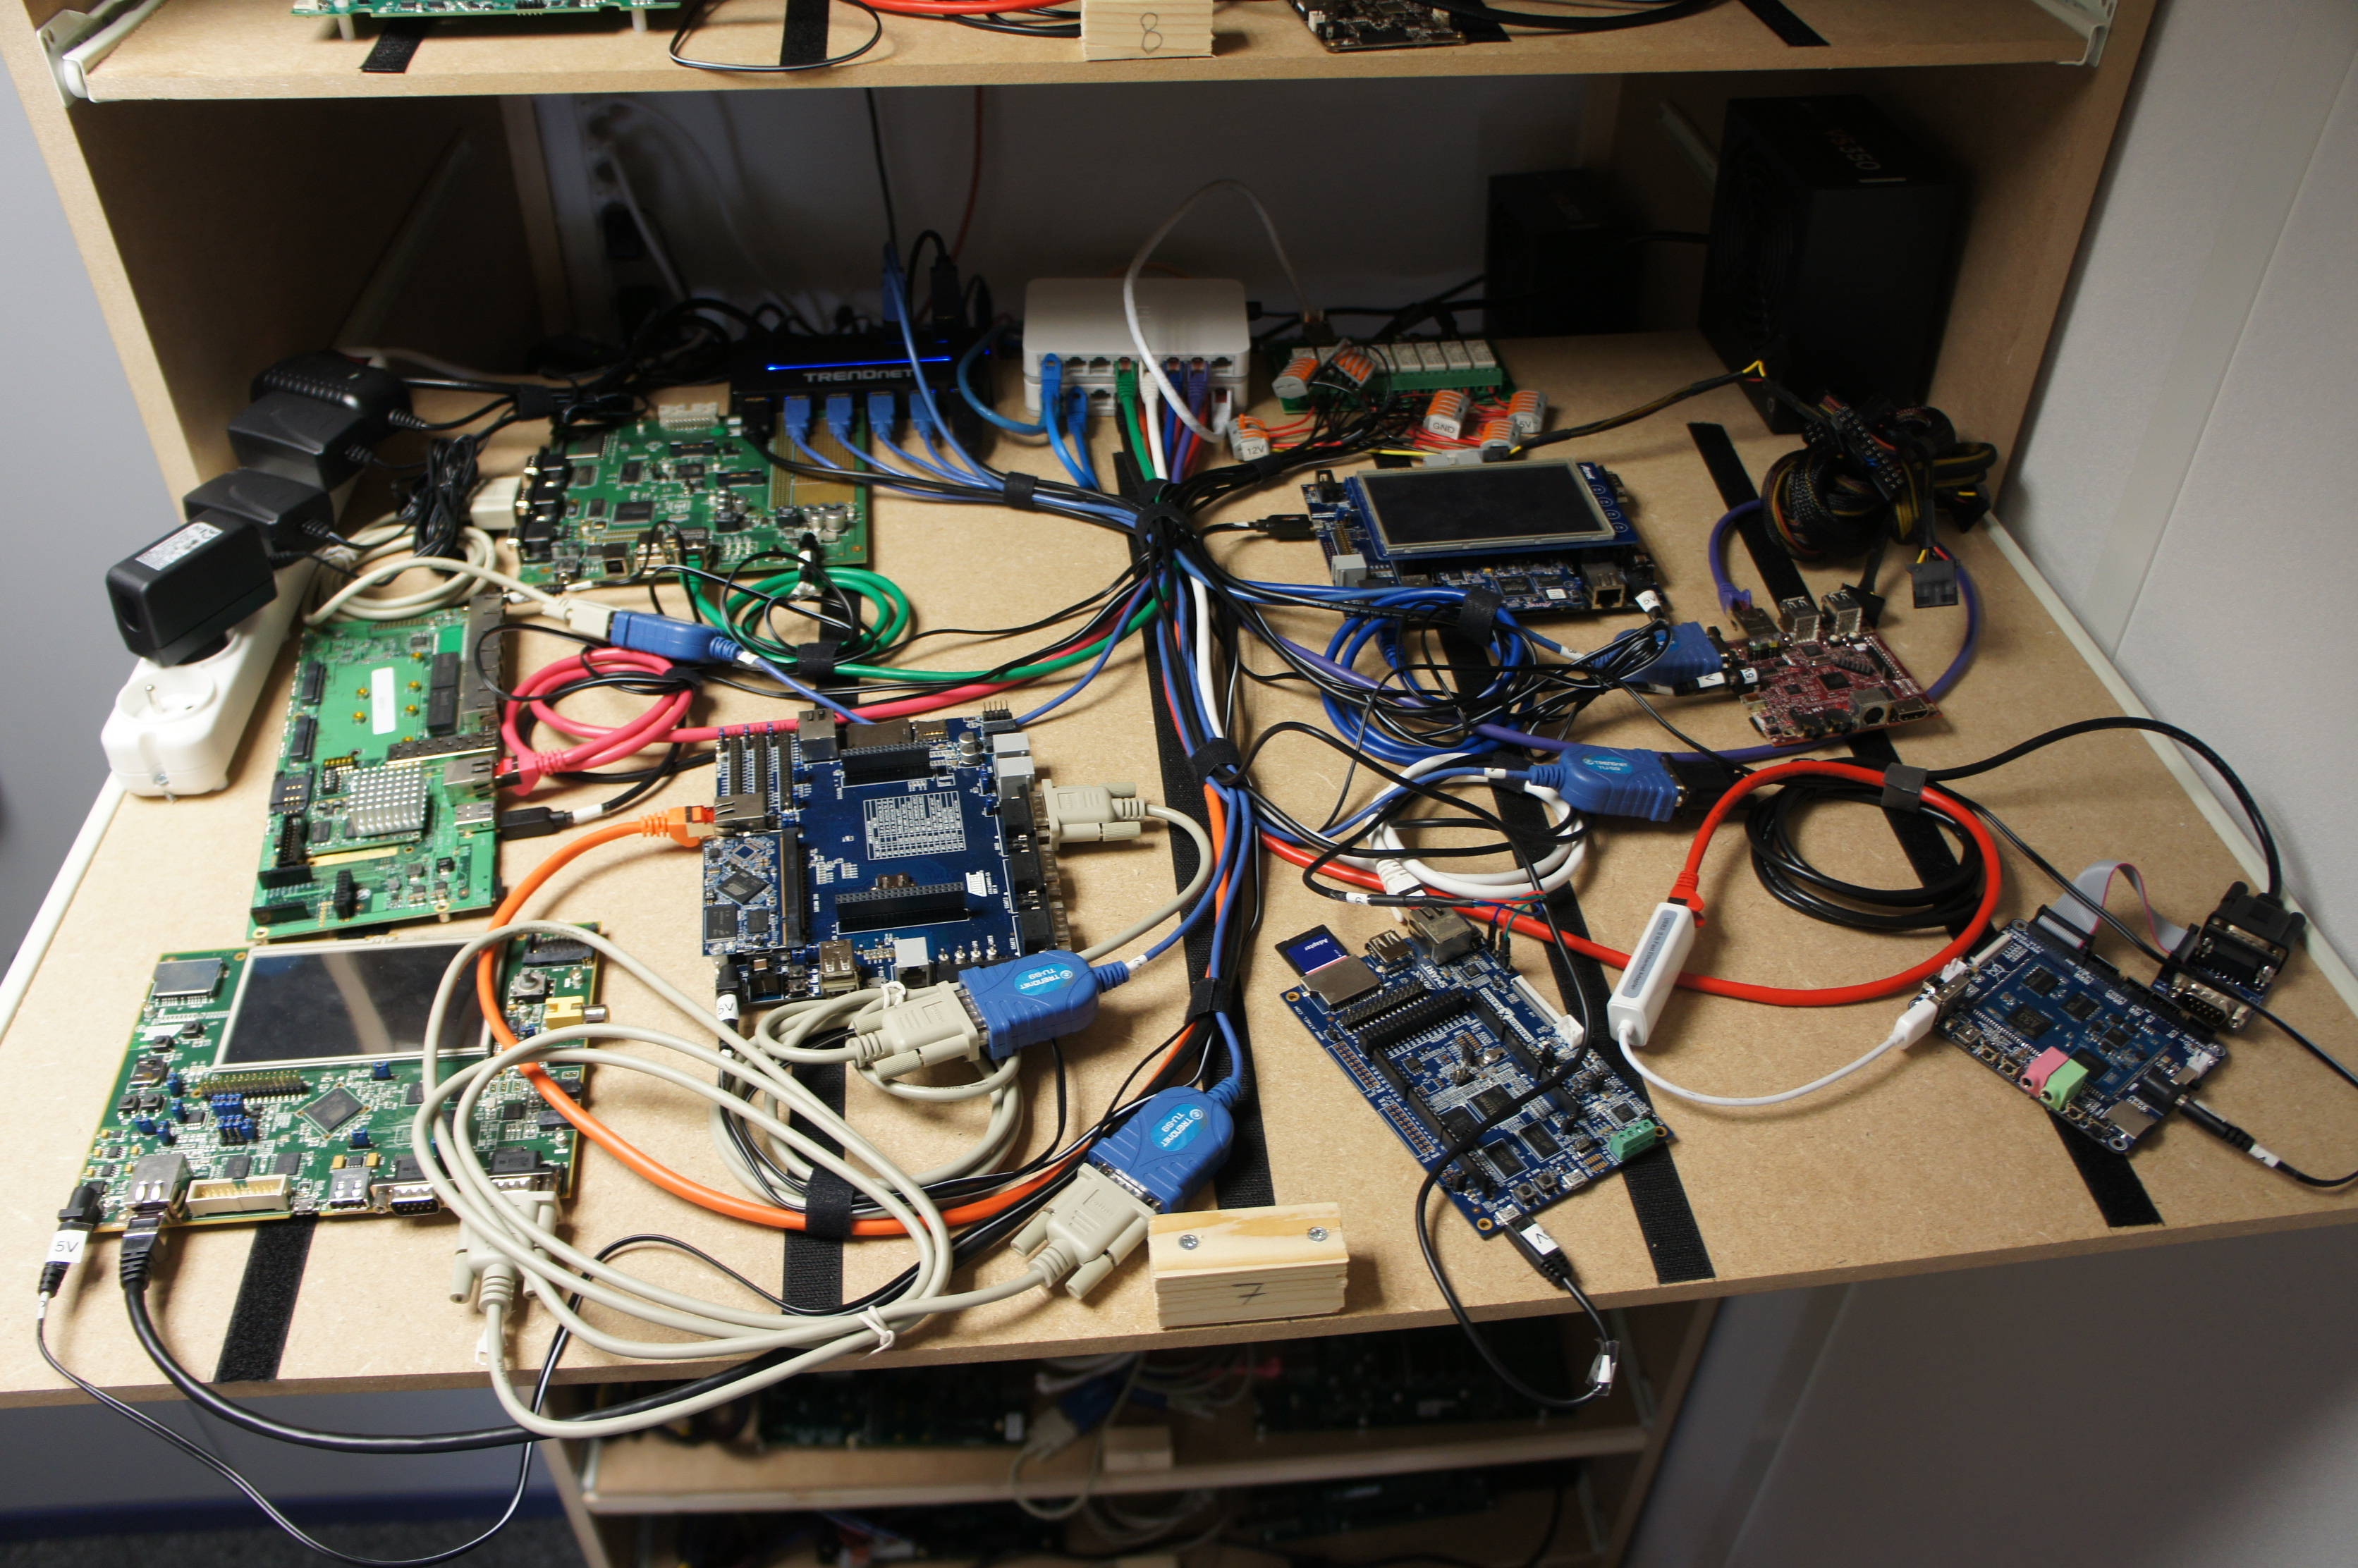
\includegraphics[width=\textwidth]{small_drawer.JPG}
  \caption{\textit{Small drawer} in the lab}
\end{figure}

\subsection{Process to add devices to the lab}

We first make sure to have a fully working bootloader on the board. This bootloader has to be accessible "hands-free" when the board has its power reset (no button should have to be pushed) or we cannot add the board to the lab. The bootloader needs TFTP (or fastboot) support to get files from the server. We then need to know where to load the kernel, DTB and initramfs in the RAM of the board. Most of the time, it is in the environment of the bootloader but we might have to take a look at the User Manual or Datasheet of our board.

Then we have to physically add the board to the lab: wire the power supply to the relay and the board, connect the serial cable to the USB hub and the board and plug an Ethernet cable in both the switch and the board. After that, we test that the serial connection pops up in our LAVA dispatcher under the device we expect thanks to our udev rules. However, some boards might expose multiple serial interfaces in Linux and we have to make sure the one we connect to is the one used to debug the board and in this case, we need to modify our generic udev rules to take into account these board-specific settings.

The last requirement before adding our board to the lab is to find a working kernel to make sure the board has booted at least once, or we would not know if it is our board's configuration or the kernel that is faulty. After a successful boot, we can install the board in the lab, add the board in LAVA and edit the scripts used by KernelCI to add support for the board\footnote{\url{https://github.com/kernelci/lava-ci\#add-board-to-kernelci}}. Then, we make sure the modifications are valid by running the script locally and sending the created jobs to our lab.

For the ATMEL AT91SAMA5D2 Xplained:
\begin{itemize}
  \item This creates jobs associated to the board in ./jobs

\begin{minted}[linenos=true,bgcolor=grey,numberblanklines=true,breaklines=true]{console}
$ ./lava-kernel-ci-job-creator.py http://storage.kernelci.org/next/next-20150114/ --plans boot --targets at91-sama5d2_xplained
\end{minted}

  \item and this will send the jobs to our LAVA server.

\begin{minted}[linenos=true,bgcolor=grey,numberblanklines=true,breaklines=true]{console}
$ ./lava-job-runner.py --username LAVA_USERNAME --token LAVA_TOKEN --server LAVA_SERVER --stream /anonymous/mybundle/
\end{minted}

  \item Then we need to follow the jobs' status and make sure they succeed before sending a patch for the added support of the board to KernelCI.
\end{itemize}

\section{Challenges encountered}
The first and most challenging problem encountered was to install LAVA whereas LAVA was migrating to a new model. For backward compatibility, LAVA has both models in the current code until it gets definitely removed in a few years. However, since LAVA developers are actively developing the new version, they did not take the time (at the time) to separate the old and new model's documentations. There were no way to distinguish which model the documentation was refering to. The main problem is KernelCI using only the old model. This cost me a lot of time to figure out why LAVA was not working in certain configurations or when following tutorials.

Among the other challenges, I had to deal with bootloaders. One of the tasks was to find the correct addresses where to load the kernel, Device Tree Blob and rootfs images in the RAM. It is often in bootloader's default configuration but sometimes I had to read the User Manual of the SoC to find at which address starts the RAM. Sometimes, even this data is not available so I had to empirically guess the address of the RAM. For some boards, the bootloader was outdated and impossible to update. Some of these bootloaders did not have bootz support, the boot method used to boot the images created when building the kernel. Instead, they have bootm support which is used to boot uImages, a format which includes the kernel and Device Tree Blob in the same image and specifies to which address in the RAM to load the uImage. Some bootloaders did not have DHCP, so we had to set fixed IP ranges for bootloaders without DHCP support.

The biggest problems I had to take care of were board-specific problems.\\
Some boards like the Marvell RD-370 need a rising edge on a pin to boot meaning we cannot avoid pressing the reset button between each boot. To work ou this problem, we had to customize the board (mainly swap resistors) to bypass this limitation.\\
Some other boards lose their serial connection. This is the heart of the continuous integration since it is the only way to communicate with the board. Some lose it when resetting their power, problem we found acceptable to solve by infinitely reconnecting to the serial. However, we still have a problem with few boards which randomly close their serial connection without any reason. After that, we are able to connect to the serial connection again but it does not send any character. The only way to get it to work again is to physically re-plug the cable used by the serial connection. Unfortunately, we did not find yet a way to solve this bug.

As detailed before, we need a serial connection for each board (up to 50) in the lab. However, the Linux kernel of our server refused to bind more than 13 USB devices when it was time to create a second drawer of boards. After some research, I found out that the culprit was the xHCI\footnote{\url{https://en.wikipedia.org/wiki/Extensible\_Host\_Controller\_Interface}} driver. In modern computers, it is possible to deactivate the support of xHCI in the BIOS but this option was not present in our server's BIOS. The solution to this problem was to rebuild and install a kernel for the server without the xHCI driver compiled. From that day, the number of USB devices is limited to 127 as in USB specification\footnote{\url{http://www.usb.org/developers/docs/usb\_31\_052016.zip}}.

\section{Conclusion}
At the end of my internship at Free Electrons, the company had a lab since May 2016 contributing to KernelCI with a pool of 20 boards (on a maximum of 50). Custom tests were unfortunately not implemented because I started to work on the subjects presented in next chapters. However, our lab performed more than 60.000 boot tests in a three months span and our engineers and more globally maintainers are using the boot reports to help themselves for support.

\subsection{Patches}

\begin{itemize}
  \item \href{https://review.linaro.org/#/q/Quentin\%20Schulz}{32 new LAVA device types configuration files},
  \item \href{https://github.com/kernelci/lava-ci/commits/master?author=quentin.schulz\%40free-electrons.com&page=1}{33 new supported devices in KernelCI},
  \item lava-ci documentation updates \href{https://github.com/kernelci/lava-ci/commit/058e9a72a752c9851c16a96aa51beafc9ce80128}{\#1}, \href{https://github.com/kernelci/lava-ci/pull/56}{\#2},
\end{itemize}
